\begin{savequote}[45mm]
\ascii{Any fool can write code that a computer can understand. Good programmers write code that humans can understand.}
\qauthor{\ascii{- Martin Flower}}
\end{savequote}

\chapter{会话} 
\label{ch:session}

\begin{content}

客户端以\code{Session}为桥梁,与后台计算引擎建立连接,并启动计算图的执行过程。其中,通过调用\code{Session.run}将触发\ascii{TensorFlow}的一次计算\ascii{(Step)}。

事实上,\code{Session}建立了执行计算图的闭包环境,它封装了\ascii{OP}计算,及其\ascii{Tensor}求值的计算环境。

\end{content}

\section{资源管理}

\begin{content}

在\code{Session}的生命周期中,将根据计算图的计算需求,按需分配系统资源,包括变量,队列,读取器等。

\subsection{关闭会话}

当计算完成后,需要确保\code{Session}被安全地关闭,以便安全释放所管理的系统资源。

\begin{leftbar}
\begin{python}
sess = tf.Session()
sess.run(targets)
sess.close()
\end{python}
\end{leftbar}

\subsection{上下文管理器}

一般地,常常使用上下文管理器创建\code{Session},使得\code{Session}在计算完成后,能够自动关闭,确保资源安全性地被释放。

\begin{leftbar}
\begin{python}
with tf.Session() as sess:
  sess.run(targets)
\end{python}
\end{leftbar}

\subsection{图实例}

一个\code{Session}实例,只能运行一个图实例;但是,一个图实例,可以运行在多个\code{Session}实例中。如果尝试在同一个\code{Session}运行另外一个图实例,必须先关闭\code{Session}(不必销毁),再启动新图的计算过程。

虽然一个\code{Session}实例,只能运行一个图实例。但是,可以\code{Session}是一个线程安全的类,可以并发地执行该图实例上的不同子图。例如,一个典型的机器学习训练模型中,可以使用同一个\code{Session}实例,并发地运行输入子图,训练子图,及其\ascii{Checkpoint}子图。

\subsubsection{引用计数器}

为了提高效率,避免计算图频繁地创建与销毁,存在一种实现上的优化技术。在图实例中维护一个\code{Session}的引用计数器,当且仅当\code{Session}的数目为零时,才真正地销毁图实例。

\begin{figure}[!htbp]
\centering
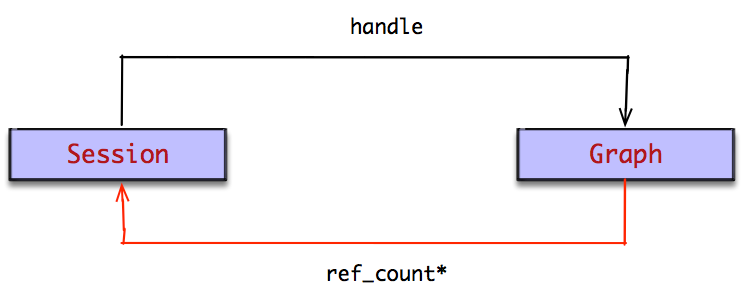
\includegraphics[width=0.7\textwidth]{figures/tf-graph-session-relation.png}
\caption{优化技术:会话实例的引用计数器}
 \label{fig:tf-graph-session-relation}
\end{figure}

\subsubsection{数据结构}

此处,摘取\code{TF\_Graph}部分关于\code{Session}引用计数器技术的关键字段;其中,\code{TF\_Graph}结构体定义于\ascii{C API}的头文件。

\begin{leftbar}
\begin{c++}
struct TF_Graph {
  TF_Graph();

  tensorflow::mutex mu;
  tensorflow::Graph graph GUARDED_BY(mu);

  // TF\_Graph may only and must be deleted when
  // num\_sessions == 0 and delete\_requested == true

  // num\_sessions incremented by TF\_NewSession, 
  // and decremented by TF\_DeleteSession.
  int num_sessions GUARDED_BY(mu);
  bool delete_requested GUARDED_BY(mu);
};
\end{c++}
\end{leftbar}

同理,\code{TF\_Session}持有一个二元组:\code{<tensorflow::Sesssion, TF\_Graph>},它们之间是一对一的关系。其中,\code{tensorflow::Sesssion}是\ascii{C++}客户端侧的会话实例。

\begin{leftbar}
\begin{c++}
struct TF_Session {
  TF_Session(tensorflow::Session* s, TF_Graph* g)
      : session(s), graph(g), last_num_graph_nodes(0) {}
  tensorflow::Session* session;
  TF_Graph* graph;
  tensorflow::mutex mu;
  int last_num_graph_nodes;
};
\end{c++}
\end{leftbar}

\subsubsection{创建会话}

\begin{leftbar}
\begin{c++}
TF_Session* TF_NewSession(TF_Graph* graph, const TF_SessionOptions* opt,
                          TF_Status* status) {
  Session* session;
  status->status = NewSession(opt->options, &session);
  if (status->status.ok()) {
    if (graph != nullptr) {
      mutex_lock l(graph->mu);
      graph->num_sessions += 1;
    }
    return new TF_Session(session, graph);
  } else {
    DCHECK_EQ(nullptr, session);
    return nullptr;
  }
}
\end{c++}
\end{leftbar}

\subsubsection{销毁会话}

\begin{leftbar}
\begin{c++}
void TF_DeleteSession(TF_Session* s, TF_Status* status) {
  status->status = Status::OK();
  TF_Graph* const graph = s->graph;
  if (graph != nullptr) {
    graph->mu.lock();
    graph->num_sessions -= 1;
    const bool del = graph->delete_requested && graph->num_sessions == 0;
    graph->mu.unlock();
    if (del) delete graph;
  }
  delete s->session;
  delete s;
}
\end{c++}
\end{leftbar}

\section{默认会话}

\begin{content}

通过调用\ascii{Session.as\_default()},将该\code{Session}置为默认\code{Session},同时它返回了一个上下文管理器。在默认\code{Session}的上文中,可以直接实施\ascii{OP}的运算,或者\ascii{Tensor}的求值。

\begin{leftbar}
\begin{python}
hello = tf.constant('hello, world')

sess = tf.Session()  
with sess.as_default():
  print(hello.eval())
sess.close()
\end{python}
\end{leftbar}

但是,\code{Session.as\_default()}并不会自动关闭\code{Session},需要用户显式地调用\code{Session.close}方法。

\subsection{张量求值}

如上例代码,\code{hello.eval()}等价于\code{tf.get\_default\_session().run(hello)}。其中,\code{Tensor.eval}如下代码实现。

\begin{leftbar}
\begin{python}
class Tensor(_TensorLike):
  def eval(self, feed_dict=None, session=None):
    if session is None:
      session = get_default_session()
    return session.run(tensors, feed_dict)
\end{python}
\end{leftbar}

\subsection{OP运算}

同理,当用户未显式提供\code{Session},\code{Operation.run}将自动获取默认的\code{Session}实例,并按照当前\ascii{OP}的依赖关系,以某个特定的拓扑排序执行该计算子图。

\begin{leftbar}
\begin{python}
class Operation(object):
  def run(self, feed_dict=None, session=None):
    if session is None:
      session = tf.get_default_session()
    session.run(self, feed_dict)
\end{python}
\end{leftbar}

\subsection{线程相关}

默认会话仅仅对当前线程有效,以便在当前线程追踪Session的调用栈。如果在新的线程中使用默认会话,需要在线程函数中通过调用\code{as\_default}将\code{Session}置为默认会话。

事实上,在\ascii{TensorFlow}运行时维护了一个\code{Session}的本地线程栈,实现默认\code{Session}的自动管理。

\begin{leftbar}
\begin{python}
_default_session_stack = _DefaultStack()

def get_default_session(session):
  return _default_session_stack.get_default(session)
\end{python}
\end{leftbar}

其中,\code{\_DefaultStack}表示栈的数据结构。

\begin{leftbar}
\begin{python}
class _DefaultStack(threading.local):
  def __init__(self):
    super(_DefaultStack, self).__init__()
    self.stack = []

  def get_default(self):
    return self.stack[-1] if len(self.stack) >= 1 else None

  @contextlib.contextmanager
  def get_controller(self, default):
    try:
      self.stack.append(default)
      yield default
    finally:
      self.stack.remove(default)
\end{python}
\end{leftbar}

\end{content}

\section{会话类型}

\begin{content}

一般地,存在两种基本的会话类型:\code{Session}与\code{InteractiveSession}。后者常常用于交互式环境,它在构造期间将其自身置为默认,简化默认会话的管理过程。

此外,两者在运行时的配置也存在差异。例如,\code{InteractiveSession}将\code{GPUOptions.allow\_growth}置为\code{True},避免在实验环境中独占整个GPU的存储资源。

\begin{figure}[!htbp]
\centering
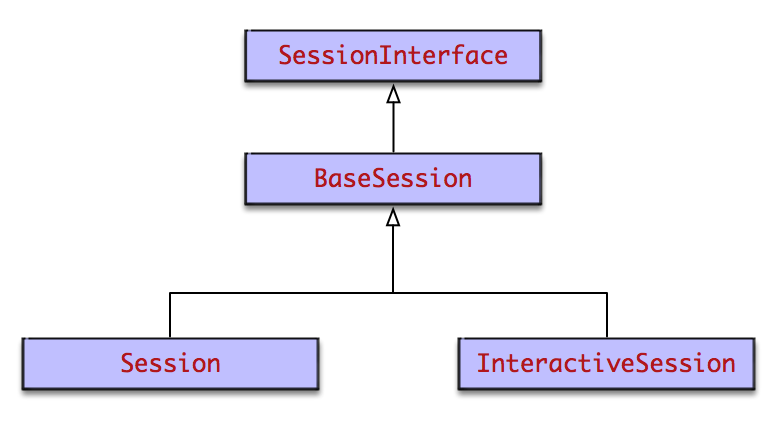
\includegraphics[width=0.7\textwidth]{figures/py-session-hierarchy.png}
\caption{Session:类层次结构}
 \label{fig:py-session-hierarchy}
\end{figure}

\subsection{Session}

\code{Session}继承\code{BaseSession},并增加了默认图与默认会话的上下文管理器的功能,保证系统资源的安全释放。

一般地,使用\code{with}进入会话的上下文管理器,并自动切换默认图与默认会话的上下文;退出\code{with}语句时,将自动关闭默认图与默认会话的上下文,并自动关闭会话。

\begin{leftbar}
\begin{python}
class Session(BaseSession):
  def __init__(self, target='', graph=None, config=None):
    super(Session, self).__init__(target, graph, config=config)
    self._default_graph_context_manager = None
    self._default_session_context_manager = None

  def __enter__(self):
    self._default_graph_context_manager = self.graph.as_default()
    self._default_session_context_manager = self.as_default()

    self._default_graph_context_manager.__enter__()
    return self._default_session_context_manager.__enter__()

  def __exit__(self, exec_type, exec_value, exec_tb):
    self._default_session_context_manager.__exit__(
        exec_type, exec_value, exec_tb)
    self._default_graph_context_manager.__exit__(
        exec_type, exec_value, exec_tb)

    self._default_session_context_manager = None
    self._default_graph_context_manager = None

    self.close()
\end{python}
\end{leftbar}

\subsection{InteractiveSession}

与\code{Session}不同,\code{InteractiveSession}在构造期间将其自身置为默认,并实现默认图与默认会话的自动切换。与此相反,\code{Session}必须借助于\code{with}语句才能完成该功能。在交互式环境中,\code{InteractiveSession}简化了用户管理默认图和默认会话的过程。

同理,\code{InteractiveSession}在计算完成后需要显式地关闭,以便安全地释放其所占用的系统资源。

\begin{leftbar}
\begin{python}
class InteractiveSession(BaseSession):
  def __init__(self, target='', graph=None, config=None):
    super(InteractiveSession, self).__init__(target, graph, config)

    self._default_session_context_manager = self.as_default()
    self._default_session_context_manager.__enter__()

    self._default_graph_context_manager = graph.as_default()
    self._default_graph_context_manager.__enter__()

  def close(self):
    super(InteractiveSession, self).close()
    self._default_graph.__exit__(None, None, None)
    self._default_session.__exit__(None, None, None)
\end{python}
\end{leftbar}

\subsection{BaseSession}

\code{BaseSession}是两者的基类,它主要实现会话的创建,关闭,执行,销毁等管理生命周期的操作;它与后台计算引擎相连接,实现前后端计算的交互。

\subsubsection{创建会话}

通过调用\ascii{C API}的接口,\code{self.\_session}直接持有后台计算引擎的会话句柄,后期执行计算图,关闭会话等操作都以此句柄为标识。

\begin{leftbar}
\begin{python}
class BaseSession(SessionInterface):
  def __init__(self, target='', graph=None, config=None):
    # ignore implements...
    with errors.raise_exception_on_not_ok_status() as status:
      self._session = 
        tf_session.TF_NewDeprecatedSession(opts, status)
\end{python}
\end{leftbar}

\subsubsection{执行计算图}

通过调用\code{run}接口,实现计算图的一次计算。它首先通过\code{tf\_session.TF\_ExtendGraph}将图注册给后台计算引擎,然后再通过调用\code{tf\_session.TF\_Run}启动计算图的执行。

\begin{leftbar}
\begin{python}
class BaseSession(SessionInterface):
  def run(self, 
    fetches, feed_dict=None, options=None, run_metadata=None):
    self._extend_graph()
    with errors.raise_exception_on_not_ok_status() as status:
      return tf_session.TF_Run(session, 
        options, feed_dict, fetch_list, 
        target_list, status, run_metadata)
  
  def _extend_graph(self):
    with errors.raise_exception_on_not_ok_status() as status:
      tf_session.TF_ExtendGraph(self._session,
        graph_def.SerializeToString(), status)  
\end{python}
\end{leftbar}

\subsubsection{关闭会话}

\begin{leftbar}
\begin{python}
class BaseSession(SessionInterface):
  def close(self):
    with errors.raise_exception_on_not_ok_status() as status:
      tf_session.TF_CloseDeprecatedSession(self._session, status)
\end{python}
\end{leftbar}

\subsubsection{销毁会话}

\begin{leftbar}
\begin{python}
class BaseSession(SessionInterface):
  def __del__(self):
    try:
      status = tf_session.TF_NewStatus()
      tf_session.TF_DeleteDeprecatedSession(self._session, status)
    finally:
      tf_session.TF_DeleteStatus(status)
\end{python}
\end{leftbar}

\begin{content}